\section{Pneumatic System}

\subsection{Purpose}

Actuation of the clutch and gear selection levers. 

Be controlled electronically by the transmission control module.


\subsection{System Overview}

\begin{figure}
\centering
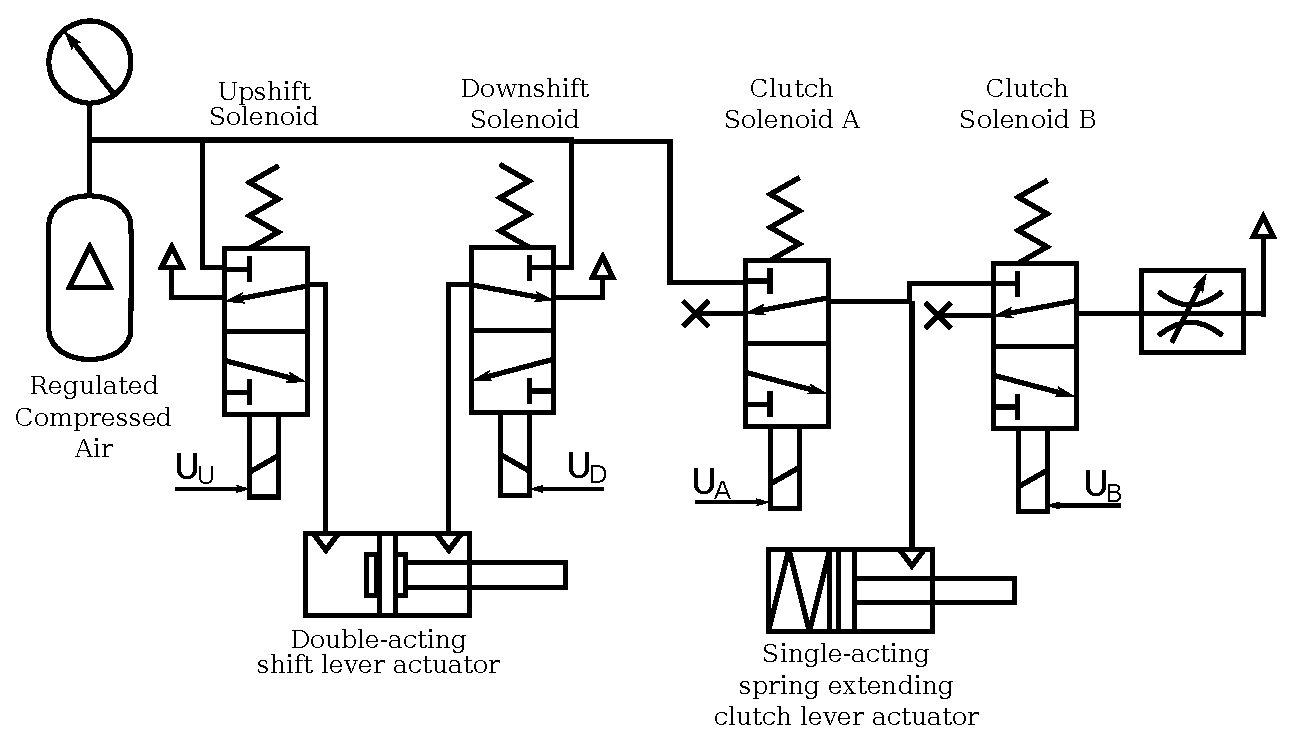
\includegraphics[scale=0.5]{design/figures/pneumatics}
\caption{Transmission control pneumatics design.}
\label{fig:pneumatics_design}
\end{figure}

After deciding to not change away from pneumatics, an improved actuation scheme was proposed that would both improve the controllability and efficiency of the system. A diagram of the mechanical portion of the pneumatics system can be seen in Figure \ref{fig:pneumatics_design}.

\subsubsection{Air tank}

An on-board compressed air tank 

\subsubsection{Regulator}

The air tank is fitted with a pressure regulator, which regulates the system pressure to approximately $120\,psi$. 

\subsubsection{Valves}

4 electronically controlled pneumatic valves control the flow of air to and from 2 pneumatic actuators.

\subsubsection{Cylinders}


\subsubsection{Mechanical Linkage }


\subsubsection{Positional Sensors }


\subsection{Valving Design}

Reduces air consumption

Increases controllability


\subsection{Modelling}

Entire system modelled in Simulink